\section{Dynamic Sub-session}

The dynamic sub-session is an integral part of the architecture. 

\subsection{Loss-Free Update}

In the protocol design, we have suspending/suspended phases, where the system stops sending traffic for migration. However, it is hard to achieve it without modifying TCP or other protocols' control logic. We need a workaround to ensure the initial deploy-ability goal: \textit{it is network protocol independent and requires no change in existing protocols}. 

To do this, we first need to understand the control logic in these protocols: there is a hash table that tracks connection and accepts flows from established connection. If we insert a middlebox protocol, this protocol translates an original flow to its sub-sessions and translate back to the original flow for the returning traffic. Moving the flow from one path to another is equivalent to updating the translation layer at the data plane. A correct update should ensure that we do not send the traffic through the new path unless the path is set up, otherwise either side will see unexpected packets and pop up error like ``\textsf{Connection reset by peers}". 

How to find the right sequence of updates for a general network is proven to be NP-complete~\cite{SWAN, zUpdate}, but for a special topology, linear in our setting, we can apply the concept from network consistent update~\cite{consistentupdate, ratul}. We first ensure that the new configurations are all pushed before the ingress applies the new configuration, and the old configurations are not removed until the egress sends the last packet. In particular, when a migration is initialized from the middlebox, it notifies its neighbor, which inserts a new translation rule for incoming traffic. Then this neighbor notifies the other side of the connection via UPDATE-SYN. Each hop receiving UPDATE-SYN updates its own translation table. Once the target host receives the notification, the new configuration will have been installed at every hop for one direction of the traffic, and thus we apply the new configuration for all new packets after the greatest sequence number seen so far. The opposite direction is set up via the same way from UPDATE-SYN-ACK. Once the old connection sees no packet for a certain period of time, e.g. a timeout, we remove the old configuration using the same mechanism. 

\textbf{Theorem:} 
The update is per-packet consistent. 

\begin{proof}
We prove by reducing the problem to a generalized consistent update~\cite{consistentupdate}. We build the case where the network has a linear topology, and each flow with five tuples has a unique rule, then the update approach is two-phase update. A two-phase update ensures per-packet consistency. 
 
\end{proof}

\begin{figure}[ht]
\centering
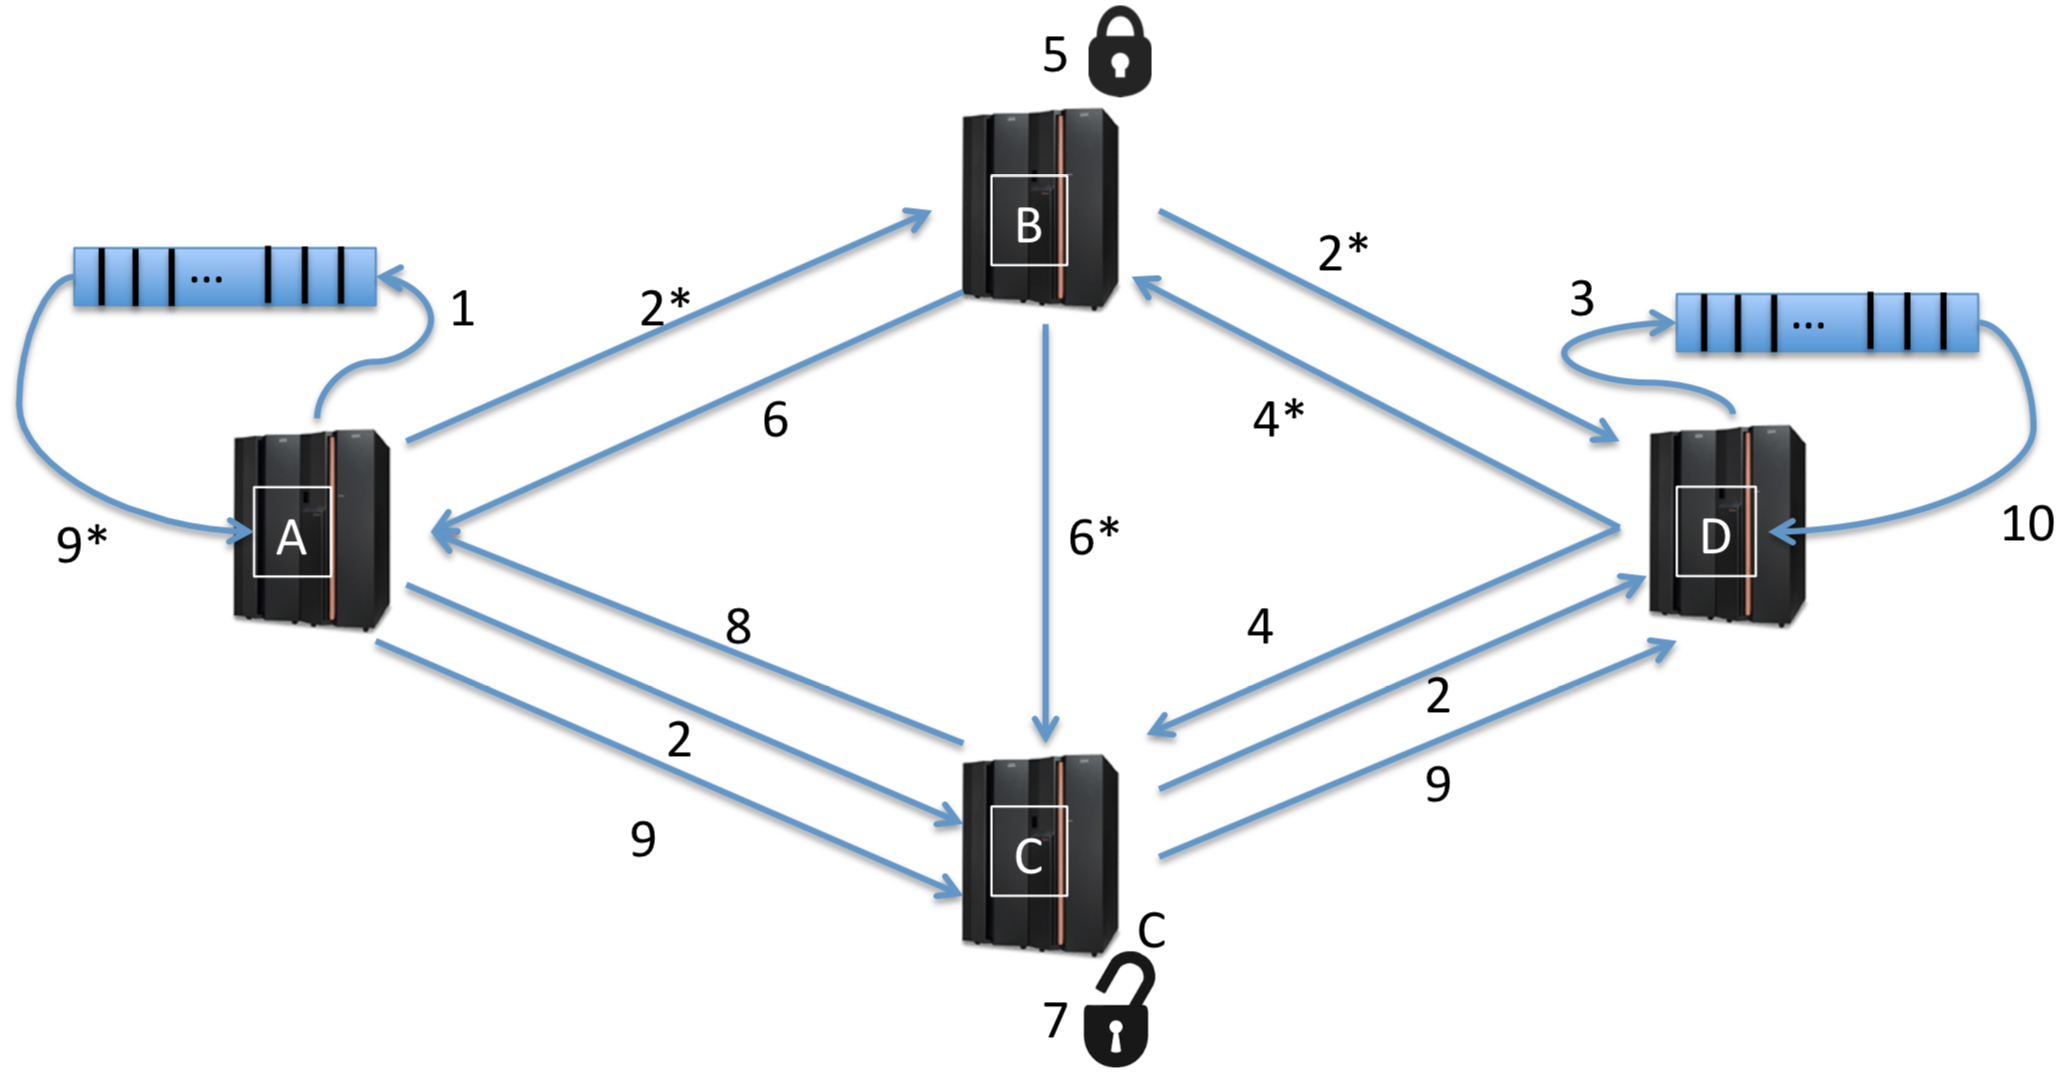
\includegraphics[width=\linewidth]{figures/order_preserving.png} 

\caption{\small We assume the migration is initiated at middlebox D, and the steps for an order-preserving update: 1. lock outgoing traffic; 2. send SYN packets; 3. lock the reverse direction traffic; 4. send SYNACK packets; 5. lock middlebox states; 6*. migrate states; 6. send SYNACK from old path; 7. finish migration and unlock states; 8. send SYNACK from new path; 9*. release buffered traffic; 9. send ACK packets; 10. release buffered traffic from the other side}\label{orderpreserving}
\end{figure}

\subsection{Traffic-Locking Update}

In a loss-free update, we keep traffic on the old path before the new path is set up. However, we may fail to migrate the flow, since this requires us to migrate middlebox state but the state cannot be moved since it is being continuously updated as the packets coming in. In this case, to lock and migrate the middlebox state we should stop sending traffic during the new path setup. Since changing the protocols (e.g., TCP and UDP) flow control logic is undesirable, we choose to buffer the traffic and not to release it until the middlebox state on the old path has been locked and replicated to the new middlebox. A fully described migration is in figure~\ref{orderpreserving}.


The definition for \textit{an order-preserving update} is that the update itself does not introduce reordering. A traffic-locking update is also order-preserving. If we assume a FIFO network with no congestion, the protocol control messages are sent after the locking of the flow, and thus it comes after the last packet sent on the path. It is safe to lock and migrate middlebox states after seeing the SYNACK packet because this packet signals both directions are locked, and thus is after the last packet sent from both directions. The update mechanism does not break the initial network semantics. (Note the mechanism does not guarantee order-preserving if the network is not FIFO or loss-free.) 

\begin{figure}[ht]
\centering
% 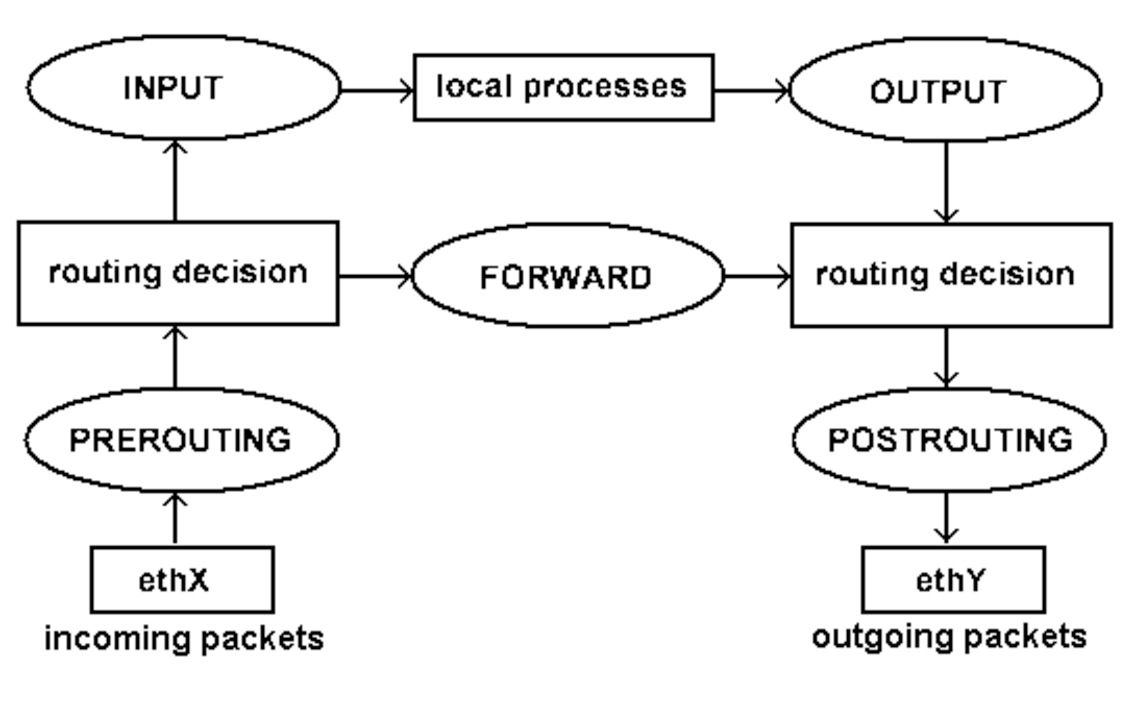
\includegraphics[scale=0.25]{figures/netfilter.pdf} 
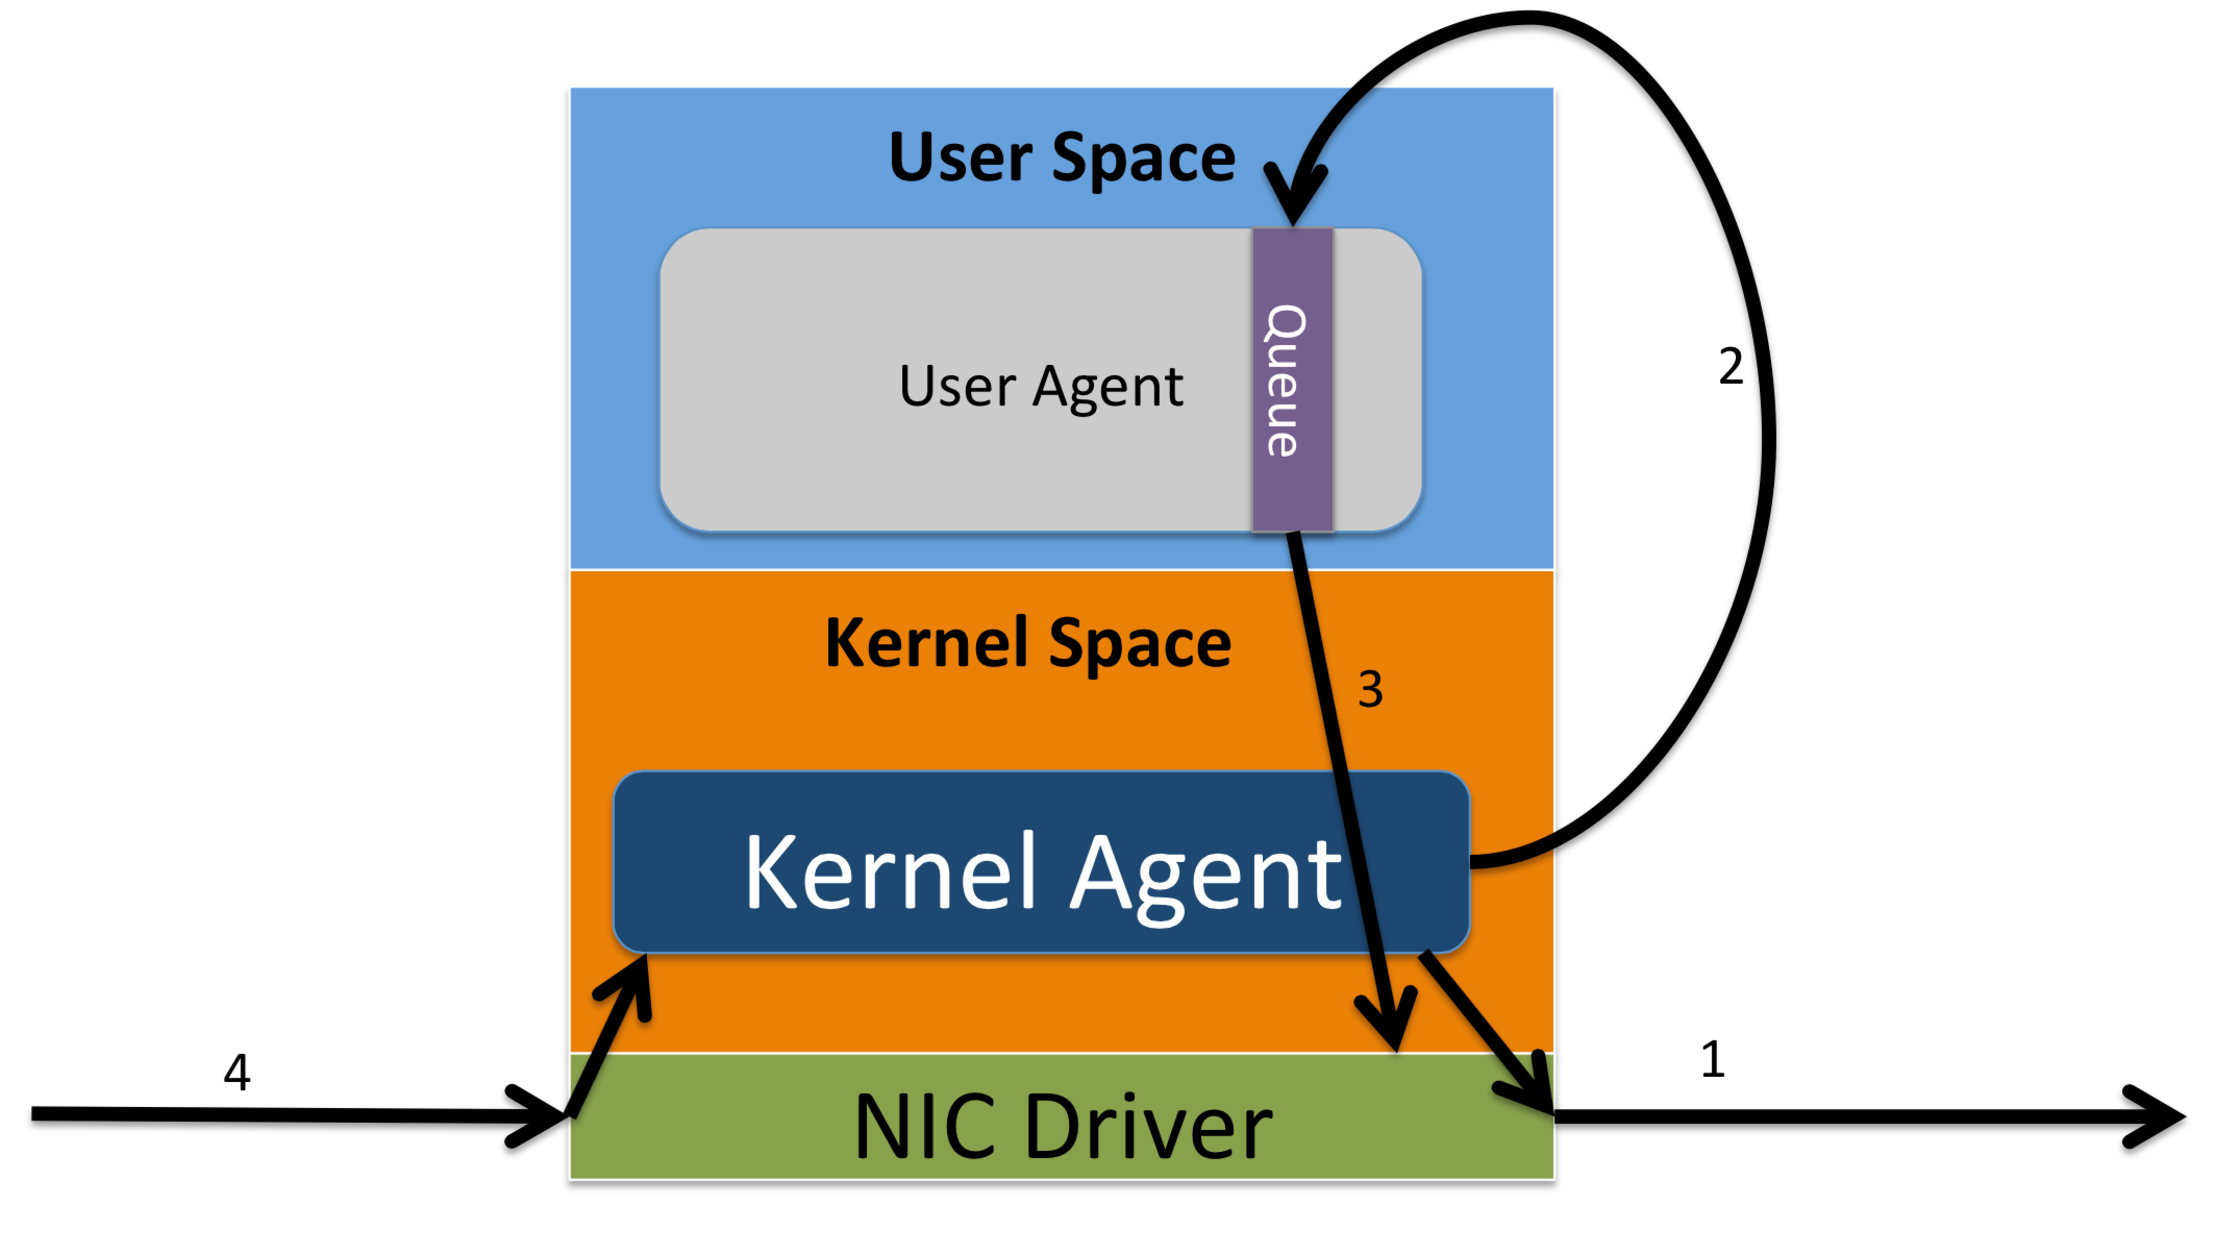
\includegraphics[width=\linewidth]{figures/flowstream.pdf} 

\caption{\small Data stream during order preserving migration: the system 1. sends out traffic through the old path, 2. buffers the packets in the user space queue, 3. receives notification from the other side and releases the buffer, and 4. directs newly coming traffic through the new path}\label{flowstream}
\end{figure}




\begin{algorithm} [ht]
\small
\SetAlgoLined

\SetKwFunction{packet}{packet\_out}\SetKwFunction{IPC}{command\_in}\SetKwFunction{queue}{Queue Agent}
\SetKwProg{mypacket}{Event\_Handler}{}{}
\SetKwProg{func}{Program}{}{}

\mypacket{\packet{} } {
lock\;
action lookup\;
\If{During Migration}{
\If{Buffer is needed}{
unlock\;
send to user queue\;
}\Else {
  \emph{Note: we do not unlock here, wait for queue to drain}\;
  mark the last packet\;
  send to user queue\;
  
  Migration = False\;
  }
} \Else{ 
  unlock\;
  send out\;
  }
  }
\mypacket{\IPC{} } {
  \If{MBP.SYN\_Update==True}
  {
  Migration = True\;
  ToBuffer = True\;
  }
  \If{MBP.ACK\_Update==True}{
  ToBuffer = False\;}
  \If{User queue is drained}{
  unlock\;
  } 
}
\func{\queue{}} {
  \If{MBP.ACK\_Update==False}{
  wait\;
  }  \Else{
    \While{queue is not empty}{
    send out\;
    \If{marked as the last packet}{
    notify kernel queue is drained\;
    }
    }
  }

} 
\caption{Order Preserving Flow Migration} \label{sync}

\end{algorithm} 


There is one more issue here we need to address: since at the high traffic rate we can only queue packets in the user space, we have an issue of synchronization between the user space queue and kernel space flow. In figure~\ref{flowstream} step 3 and step 4 may be interleaved, which breaks the initial network semantics. One solution is to keep the queue and enqueue all packets, however this severely penalizes the general case where the system is not in an update phase. To address this issue, we decide to take advantage of the spin\_lock for the hash table lookup, and lock the packet\_out interrupt if the user queue is not drained yet. A complete algorithm is in algorithm~\ref{sync}, and to add concurrency, we can have a flow to lock for each flow and add another lock lookup beforehand. 



\begin{comment}
\begin{algorithm} [ht]
\tiny
\SetAlgoLined
\SetKwFunction{packet}{packet\_out}\SetKwFunction{IPC}{command\_in}
\SetKwProg{mypacket}{Event\_Handler}{}{}
\mypacket{\packet{} } {

\nl Lock()\;
\nl action lookup\;
\nl Send\_out()\;
\nl Unlock()\;
}
\mypacket{\IPC{} } {
  \If{MBP.SYN\_Update==True}
  {
  \nl Lock()\;
  \nl Update action\;
  }
  \If{MBP.ACK\_Update==True}{
  \nl Unlock()\;
  } 
}

\caption{A naive solution} \label{wrongalgorithm}
\end{algorithm} 

A naive solution like algorithm~\ref{wrongalgorithm} should guarantee the synchronization in theory. However, it does not work well in practice, since interrupt-disallowed spin lock would lock the thread in the top half of Linux kernel, this can be very problematic if we have long update or timeout (e.g., $>100 ms$ ), and the NIC may drop the packets if they are not handled by kernel in time, to accept new packets.
\end{comment}


